\section{5.5 Discrete Kalman filter}
\subsection{A, Discretization of the state space model}
Discretizing a linear system, given the continuous system, is easily done with MATLAB. we have the continuous state space model from \eqref{eq:54aModel} in \autoref{seq:54a}. A sampling frequency of  $10 \si{\hertz}$ gives an sampling time of $0.1 \si{\second}$. The output matrices $C$ and $D$ remain unchanged under discretization as the relationship between the state and output does not change. We also have to use the \lstinline{c2d}-function twice, because it only accepts one input to the system. This is fine because the system is linear and the superposition principle holds. The discrete state space model can thus be found as in \autoref{lst:c2d}.
\begin{lstlisting}[caption={MATLAB script to find discretize a continuous state space model.}, label={lst:c2d}]
T_s = 0.1;
[~, Bd] = c2d(A,B,T_s);
[Ad, Ed] = c2d(A,E,T_s);
Cd = C;
Dd = D;
\end{lstlisting}
This results in the following discretized system
\begin{subequations}
\begin{align}
    \mathbf{A_d} &= 
    \begin{bmatrix}
        0.9969 & 0.1006 & 0 & 0 & 0\\
        -0.0616 & 1.0111 & 0 & 0 & 0\\
        0 & 0 & 1.0000 & 0.0999 & 0\\
        0 & 0 & 0 & 0.9986 & -0.0002\\
        0 & 0 & 0 & 0 & 1.0000
    \end{bmatrix}\\
    \mathbf{B_d} &= 
    \begin{bmatrix}
        0\\
        0\\
        1.09\cdot 10^{-5}\\
        2.173\cdot 10^{-4}\\
        0
    \end{bmatrix}\\
    \mathbf{E_d} &= 
    \begin{bmatrix}
        0 & 0\\
        0.0004 & 0\\
        0 & 0\\
        0 & 0\\
        0 & 0.1000
    \end{bmatrix}
\end{align}
\end{subequations}
\subsection{B, Estimating the variance of the measurement noise}
To estimate the variance of the measurement noise, we simulate the ship model and export the measurement noise to the MATLAB workspace as a time series. The MATLAB function \lstinline{var} can then be used to find the empirical variance. The ship model gives a measurement error in degrees, but we want to use radians in our Kalman filter implementation. The full expression is thus \lstinline{variance = var(measurement_noise*pi/180)}.

\subsection{C, Implementation of the Kalman filter}
The Kalman filter was implemented as a S-function in MATLAB. The full implementation is given in \autoref{lst:DiskKal}.

\subsection{D, Simulation with bias from the Kalman filter}
Using the estimated bias in a feed forward to to the rudder input we manage to remove the stationary deviation. Without the feed forward from the estimator the stationary deviation was significant, as seen in \autoref{fig:p3pc_rudder_heading}. \autoref{fig:p5d_rudder_heading} shows that the estimate for the bias current converges fairly quickly and we are thus able to correct the input rudder angle to remove any stationary deviation. 

\begin{figure}
    \centering
    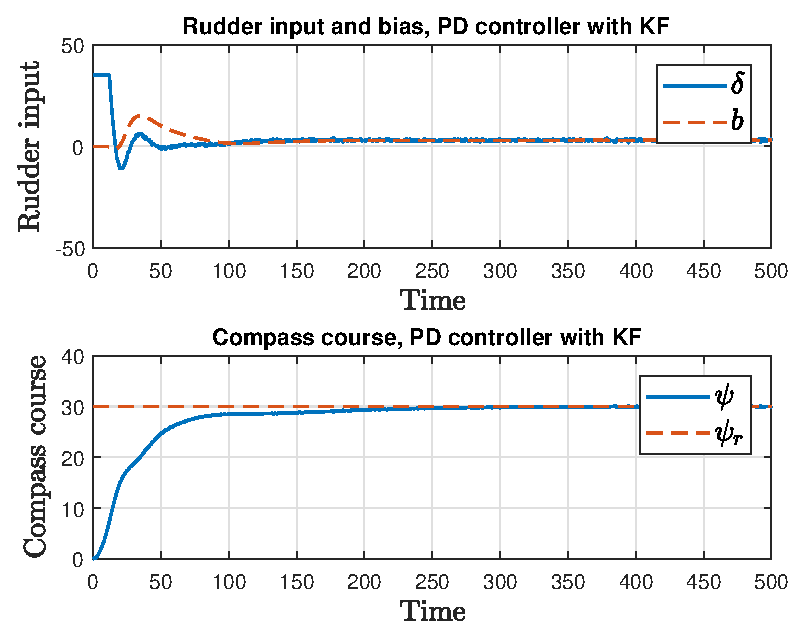
\includegraphics[width = 1.00\textwidth]{figures/plots/P5p5d_rudder_heading.eps}
    \caption{Rudder input together with bias estimate from KF and compass course of ship}
    \label{fig:p5d_rudder_heading}
\end{figure}

\subsection{E, Simulation with heading and bias from the Kalman filter}
Using the filtered heading instead of the measurement does not give a significantly better performance. The response is more oscillatory before reaching the setpoint, but is less oscillatory once the setpoint is reached.
\todo{The response should probably be better.}


\todo{Include plots of both measured and filtered compass course, rudder input and
estimated bias. Also include plots of actual wave influence and estimated wave
influence.}

\subsection{F, Discussion of the Q matrix}
The $\mathbf{Q}$ matrix is the disturbance covariance. A large $\mathbf{Q}$ represent a large disturbance, the noise greatly impacts the state. The $\mathbf{Q}$ matrix given in the assignment text is
\begin{align*}
    \mathbf{Q} &= 
    \begin{bmatrix}
        30 & 0\\
        0 & 10^{-6}
    \end{bmatrix}
\end{align*}
We see that the wave disturbance affects the system orders of magnitude more than the current disturbance.
If we were to increase the $\mathbf{Q}$ matrix we would be telling the Kalman filter that the measurements are more uncertain and they need to be filtered more.


\todo{How does changing the Q matrix affect the response in task d) and e)? Discuss why.}